% Options for packages loaded elsewhere
% Options for packages loaded elsewhere
\PassOptionsToPackage{unicode}{hyperref}
\PassOptionsToPackage{hyphens}{url}
%
\documentclass[
  ignorenonframetext,
  aspectratio=169,
]{beamer}
\newif\ifbibliography
\usepackage{pgfpages}
\setbeamertemplate{caption}[numbered]
\setbeamertemplate{caption label separator}{: }
\setbeamercolor{caption name}{fg=normal text.fg}
\beamertemplatenavigationsymbolsempty
% remove section numbering
\setbeamertemplate{part page}{
  \centering
  \begin{beamercolorbox}[sep=16pt,center]{part title}
    \usebeamerfont{part title}\insertpart\par
  \end{beamercolorbox}
}
\setbeamertemplate{section page}{
  \centering
  \begin{beamercolorbox}[sep=12pt,center]{section title}
    \usebeamerfont{section title}\insertsection\par
  \end{beamercolorbox}
}
\setbeamertemplate{subsection page}{
  \centering
  \begin{beamercolorbox}[sep=8pt,center]{subsection title}
    \usebeamerfont{subsection title}\insertsubsection\par
  \end{beamercolorbox}
}
% Prevent slide breaks in the middle of a paragraph
\widowpenalties 1 10000
\raggedbottom
\usepackage{iftex}
\ifPDFTeX
  \usepackage[T1]{fontenc}
  \usepackage[utf8]{inputenc}
  \usepackage{textcomp} % provide euro and other symbols
\else % if luatex or xetex
  \usepackage{unicode-math} % this also loads fontspec
  \defaultfontfeatures{Scale=MatchLowercase}
  \defaultfontfeatures[\rmfamily]{Ligatures=TeX,Scale=1}
\fi
\usepackage{lmodern}

\usetheme[]{metropolis}
\ifPDFTeX\else
  % xetex/luatex font selection
\fi
% Use upquote if available, for straight quotes in verbatim environments
\IfFileExists{upquote.sty}{\usepackage{upquote}}{}
\IfFileExists{microtype.sty}{% use microtype if available
  \usepackage[]{microtype}
  \UseMicrotypeSet[protrusion]{basicmath} % disable protrusion for tt fonts
}{}
\makeatletter
\@ifundefined{KOMAClassName}{% if non-KOMA class
  \IfFileExists{parskip.sty}{%
    \usepackage{parskip}
  }{% else
    \setlength{\parindent}{0pt}
    \setlength{\parskip}{6pt plus 2pt minus 1pt}}
}{% if KOMA class
  \KOMAoptions{parskip=half}}
\makeatother


\usepackage{longtable,booktabs,array}
\usepackage{calc} % for calculating minipage widths
\usepackage{caption}
% Make caption package work with longtable
\makeatletter
\def\fnum@table{\tablename~\thetable}
\makeatother
\usepackage{graphicx}
\makeatletter
\newsavebox\pandoc@box
\newcommand*\pandocbounded[1]{% scales image to fit in text height/width
  \sbox\pandoc@box{#1}%
  \Gscale@div\@tempa{\textheight}{\dimexpr\ht\pandoc@box+\dp\pandoc@box\relax}%
  \Gscale@div\@tempb{\linewidth}{\wd\pandoc@box}%
  \ifdim\@tempb\p@<\@tempa\p@\let\@tempa\@tempb\fi% select the smaller of both
  \ifdim\@tempa\p@<\p@\scalebox{\@tempa}{\usebox\pandoc@box}%
  \else\usebox{\pandoc@box}%
  \fi%
}
% Set default figure placement to htbp
\def\fps@figure{htbp}
\makeatother





\setlength{\emergencystretch}{3em} % prevent overfull lines

\providecommand{\tightlist}{%
  \setlength{\itemsep}{0pt}\setlength{\parskip}{0pt}}



 


% ============================================================
%  Econ 2203 — Beamer Metropolis Theme Preamble
%  Course: International Trade and Policy in Agriculture
%  Instructor: Nithin M, Department of Development Economics
% ============================================================

% MUST be first: load Metropolis theme before \metroset and colour overrides
\usetheme{metropolis}

% Only load packages not already provided by pandoc's beamer template
\usepackage{amsmath,amssymb}

% ---- Brand colours -----------------------------------------
\definecolor{brandblue}{HTML}{012169}
\definecolor{brandgold}{HTML}{B9975B}
\definecolor{lightblue}{HTML}{E8EDF5}

% ---- Metropolis colour overrides ---------------------------
% Main palette
\setbeamercolor{normal text}{fg=black,bg=white}
\setbeamercolor{alerted text}{fg=brandgold}
\setbeamercolor{example text}{fg=brandblue!70!black}

% Title slide
\setbeamercolor{title}{fg=white,bg=brandblue}
\setbeamercolor{subtitle}{fg=brandgold}
\setbeamercolor{author}{fg=white}
\setbeamercolor{institute}{fg=brandgold!80!white}
\setbeamercolor{date}{fg=white}
\setbeamercolor{title page header}{fg=white,bg=brandblue}

% Frametitle bar
\setbeamercolor{frametitle}{fg=white,bg=brandblue}

% Progress bar → gold
\setbeamercolor{progress bar}{fg=brandgold,bg=brandblue!30}
\setbeamercolor{title separator}{fg=brandgold}
\setbeamercolor{progress bar in head/foot}{fg=brandgold,bg=brandblue!20}
\setbeamercolor{progress bar in section page}{fg=brandgold,bg=brandblue!20}

% Blocks
\setbeamercolor{block title}{bg=brandblue,fg=white}
\setbeamercolor{block body}{bg=lightblue,fg=black}
\setbeamercolor{block title alerted}{bg=brandgold,fg=white}
\setbeamercolor{block body alerted}{bg=brandgold!12,fg=black}
\setbeamercolor{block title example}{bg=brandblue!70!black,fg=white}
\setbeamercolor{block body example}{bg=brandblue!8,fg=black}

% Structure / lists
\setbeamercolor{structure}{fg=brandblue}
\setbeamercolor{section in toc}{fg=brandblue}
\setbeamercolor{itemize item}{fg=brandblue}
\setbeamercolor{itemize subitem}{fg=brandgold}
\setbeamercolor{enumerate item}{fg=brandblue}
\setbeamercolor{description item}{fg=brandblue}

% ---- Metropolis options ------------------------------------
\metroset{
  progressbar    = frametitle,   % gold bar under frametitle
  sectionpage    = none,
  numbering      = fraction,
  block          = fill
}

% ---- Fonts (Metropolis uses Fira Sans; fallback gracefully) -
\setbeamerfont{title}{size=\Large,series=\bfseries}
\setbeamerfont{subtitle}{size=\normalsize,series=\mdseries}
\setbeamerfont{frametitle}{size=\large,series=\bfseries}
\setbeamerfont{block title}{size=\normalsize,series=\bfseries}
\setbeamerfont{caption}{size=\footnotesize}

% ---- Footer: course info + slide number --------------------
\setbeamertemplate{footline}{%
  \begin{beamercolorbox}[wd=\paperwidth,ht=2.0ex,dp=1ex]{footline}%
    \hspace{0.8em}%
    {\footnotesize\color{brandblue!60}%
      Econ 2203 \textbar{} International Trade and Policy in Agriculture
      \hfill Nithin M \hfill
      \insertframenumber{}/\inserttotalframenumber\hspace{0.8em}}%
  \end{beamercolorbox}%
}

% ---- Misc --------------------------------------------------
\setlength{\parskip}{0.25em}
\setbeamertemplate{navigation symbols}{}

% tighter column sep for side-by-side content
\setlength{\columnsep}{0.8em}

% Prevent figures from overflowing Beamer frames.
% width=\linewidth: scale to text width (already Quarto default);
% height=0.6\textheight: cap height so figures never push past the frame bottom.
% keepaspectratio: never distort — whichever constraint binds first wins.
\setkeys{Gin}{width=\linewidth,height=0.6\textheight,keepaspectratio}
\makeatletter
\@ifpackageloaded{caption}{}{\usepackage{caption}}
\AtBeginDocument{%
\ifdefined\contentsname
  \renewcommand*\contentsname{Table of contents}
\else
  \newcommand\contentsname{Table of contents}
\fi
\ifdefined\listfigurename
  \renewcommand*\listfigurename{List of Figures}
\else
  \newcommand\listfigurename{List of Figures}
\fi
\ifdefined\listtablename
  \renewcommand*\listtablename{List of Tables}
\else
  \newcommand\listtablename{List of Tables}
\fi
\ifdefined\figurename
  \renewcommand*\figurename{Figure}
\else
  \newcommand\figurename{Figure}
\fi
\ifdefined\tablename
  \renewcommand*\tablename{Table}
\else
  \newcommand\tablename{Table}
\fi
}
\@ifpackageloaded{float}{}{\usepackage{float}}
\floatstyle{ruled}
\@ifundefined{c@chapter}{\newfloat{codelisting}{h}{lop}}{\newfloat{codelisting}{h}{lop}[chapter]}
\floatname{codelisting}{Listing}
\newcommand*\listoflistings{\listof{codelisting}{List of Listings}}
\makeatother
\makeatletter
\makeatother
\makeatletter
\@ifpackageloaded{caption}{}{\usepackage{caption}}
\@ifpackageloaded{subcaption}{}{\usepackage{subcaption}}
\makeatother

\usepackage{bookmark}
\IfFileExists{xurl.sty}{\usepackage{xurl}}{} % add URL line breaks if available
\urlstyle{same}
\hypersetup{
  pdftitle={Lecture 12: Foreign Exchange Market --- Instruments and Policy},
  pdfauthor={Nithin M},
  hidelinks,
  pdfcreator={LaTeX via pandoc}}


\title{Lecture 12: Foreign Exchange Market --- Instruments and Policy}
\subtitle{Econ 2203 \textbar{} International Trade and Policy in
Agriculture}
\author{Nithin M}
\date{2026-07-11}
\institute{Department of Development Economics}

\begin{document}
\frame{\titlepage}


\begin{frame}{Forex Market: Exchange Rate Systems and Open Economy
Macro}
\phantomsection\label{forex-market-exchange-rate-systems-and-open-economy-macro}
From exchange rate regimes to the Mundell-Fleming model --- how monetary
and fiscal policy interact with the exchange rate, and what this means
for agricultural exporters and importers.
\end{frame}

\begin{frame}{Recap (Lecture 11): key equations}
\phantomsection\label{recap-lecture-11-key-equations}
\[e = \frac{\text{domestic currency}}{\text{foreign currency}}\]

\begin{itemize}
\tightlist
\item
  Absolute PPP: \(e = \frac{P_d}{P_f}\)
\item
  Relative PPP: \(\frac{\Delta e}{e} = \pi_d - \pi_f\)
\item
  UIP: \(i = i^* + \frac{E(e_{t+1}) - e_t}{e_t}\)
\end{itemize}
\end{frame}

\begin{frame}{Recap: India numerical context (illustrative)}
\phantomsection\label{recap-india-numerical-context-illustrative}
\begin{itemize}
\tightlist
\item
  INR/USD spot ≈ \textbf{₹83.5/\$}
\item
  India CPI inflation ≈ 5--6\%; US ≈ 2--3\%
\item
  Relative PPP → \textbf{\textasciitilde3--4\%} annual INR depreciation
\item
  Repo rate ≈ \textbf{6.5\%}; Fed funds ≈ \textbf{5.25--5.5\%}
\end{itemize}
\end{frame}

\begin{frame}{Today (Lecture 12): what we add}
\phantomsection\label{today-lecture-12-what-we-add}
\begin{itemize}
\tightlist
\item
  Exchange rate regimes (fixed vs float vs managed)
\item
  Mundell--Fleming: policy under different regimes
\item
  RBI intervention and reserves logic
\item
  Forward markets + hedging for agri trade
\end{itemize}
\end{frame}

\begin{frame}{Exchange Rate Systems (I): Free Float and Managed Float}
\phantomsection\label{exchange-rate-systems-i-free-float-and-managed-float}
\begin{longtable}[]{@{}
  >{\raggedright\arraybackslash}p{(\linewidth - 4\tabcolsep) * \real{0.2105}}
  >{\raggedright\arraybackslash}p{(\linewidth - 4\tabcolsep) * \real{0.3421}}
  >{\raggedright\arraybackslash}p{(\linewidth - 4\tabcolsep) * \real{0.4474}}@{}}
\toprule\noalign{}
\begin{minipage}[b]{\linewidth}\raggedright
System
\end{minipage} & \begin{minipage}[b]{\linewidth}\raggedright
Description
\end{minipage} & \begin{minipage}[b]{\linewidth}\raggedright
India Relevance
\end{minipage} \\
\midrule\noalign{}
\endhead
\textbf{Free float} & Market determines exchange rate; central bank does
not intervene & USA, UK, Eurozone --- India's major trading partners
operate under this system \\
\textbf{Managed float} & CB intervenes to smooth volatility but does not
target a specific level & \textbf{India's current system} (since 1993
post-LERMS); RBI smooths but allows gradual adjustment \\
\bottomrule\noalign{}
\end{longtable}

\textbf{India's choice:} Managed float since 1993 (post-LERMS). RBI
intervenes to smooth but does not target a specific level. This
preserves monetary policy independence while preventing destabilising
volatility.
\end{frame}

\begin{frame}{Exchange Rate Systems (II): Fixed and Intermediate
Regimes}
\phantomsection\label{exchange-rate-systems-ii-fixed-and-intermediate-regimes}
\begin{longtable}[]{@{}
  >{\raggedright\arraybackslash}p{(\linewidth - 4\tabcolsep) * \real{0.2105}}
  >{\raggedright\arraybackslash}p{(\linewidth - 4\tabcolsep) * \real{0.3421}}
  >{\raggedright\arraybackslash}p{(\linewidth - 4\tabcolsep) * \real{0.4474}}@{}}
\toprule\noalign{}
\begin{minipage}[b]{\linewidth}\raggedright
System
\end{minipage} & \begin{minipage}[b]{\linewidth}\raggedright
Description
\end{minipage} & \begin{minipage}[b]{\linewidth}\raggedright
India Relevance
\end{minipage} \\
\midrule\noalign{}
\endhead
\textbf{Crawling peg} & Regular small, pre-announced adjustments to the
peg & Chile historically; some SAARC neighbours use variants \\
\textbf{Fixed/pegged} & CB maintains exchange rate at a predetermined
target using reserves & Gulf states (USD peg); pre-1991 India maintained
a \emph{de facto} fixed rate \\
\textbf{Currency board} & 100\% foreign reserve backing for domestic
currency at fixed rate & Argentina 1991--2001 (collapsed); Hong Kong
(ongoing) \\
\textbf{Currency union} & Single shared currency across multiple
countries & Eurozone; CFA Franc zone in West/Central Africa \\
\bottomrule\noalign{}
\end{longtable}

\textbf{Historical lesson for India:} India maintained a \emph{de facto}
fixed rate through the 1980s. By 1991: BoP crisis forced a 44\%
devaluation. Post-crisis shift to managed float was the correct policy
response.
\end{frame}

\begin{frame}{Fixed exchange rate: pros and cons (agriculture)}
\phantomsection\label{fixed-exchange-rate-pros-and-cons-agriculture}
\begin{itemize}
\tightlist
\item
  Predictable rate helps long contracts (exports/imports)
\item
  Can discipline inflation (money creation constrained)
\item
  Risk of \textbf{overvaluation} → sudden crisis + forced devaluation
\item
  Monetary policy autonomy is limited
\item
  Requires reserves to defend the peg
\end{itemize}
\end{frame}

\begin{frame}{Flexible exchange rate: pros and cons (agriculture)}
\phantomsection\label{flexible-exchange-rate-pros-and-cons-agriculture}
\begin{itemize}
\tightlist
\item
  Automatic adjustment via depreciation/appreciation
\item
  Monetary policy has more room
\item
  Volatility creates pricing risk for traders
\item
  Depreciation raises costs of key imports (oil, fertiliser, edible
  oils)
\end{itemize}
\end{frame}

\begin{frame}{Case Study: India's 1991 Exchange Rate Crisis}
\phantomsection\label{case-study-indias-1991-exchange-rate-crisis}
\textbf{India's 1991 crisis --- the case for managed float:}

India maintained a \emph{de facto} fixed rate through the 1980s. By
1991: BoP deficit widened, reserves fell to \$1.2B (barely 2 weeks of
import cover), credit rating downgraded. India was forced to
\textbf{devalue 44\% in two days} (July 1--3, 1991). Post-crisis, India
adopted the Liberalised Exchange Rate Management System (LERMS) in 1992,
transitioning to a managed float by 1993. The lesson: a fixed rate
without adequate reserves and fiscal discipline is a crisis waiting to
happen.
\end{frame}

\begin{frame}{The Impossible Trinity: Statement and Intuition}
\phantomsection\label{the-impossible-trinity-statement-and-intuition}
\textbf{Statement:} A country \textbf{CANNOT} simultaneously maintain
all three of:

\begin{enumerate}
\tightlist
\item
  🔒 \textbf{Fixed exchange rate} (\(e = \bar{e}\))
\item
  🌐 \textbf{Free capital mobility} (\(CF\) unconstrained)
\item
  🏦 \textbf{Independent monetary policy} (\(i \neq i^*\))
\end{enumerate}

\textbf{Mathematical intuition:} Under a fixed rate (\(e = \bar{e}\))
and free capital (\(CF\) unconstrained), UIP forces \(i = i^*\). Then
monetary policy (\(M\)) cannot change \(i\) independently --- any
attempt to lower \(i\) below \(i^*\) triggers capital outflow, forcing
the CB to sell reserves to defend the peg, which contracts \(M\) back.

\[\{e_{\text{fixed}}\} \cup \{CF_{\text{free}}\} \cup \{MP_{\text{independent}}\}: \text{ choose any TWO}\]

\textbf{India's trilemma choice:} Managed float (partial exchange rate
flexibility) + selective capital controls (FPI restrictions, ECB limits)
= partial monetary independence. A pragmatic middle path.
\end{frame}

\begin{frame}{The Impossible Trinity: Country Examples}
\phantomsection\label{the-impossible-trinity-country-examples}
\begin{longtable}[]{@{}llll@{}}
\toprule\noalign{}
Country & Fixed rate? & Free capital? & Monetary independence? \\
\midrule\noalign{}
\endhead
USA (free float) & ✗ & ✓ & ✓ \\
Eurozone & ✓ (intra-EU) & ✓ & ✗ \\
China (capital controls) & ✓ & ✗ & ✓ \\
India (managed float) & Partial & Partial & Partial \\
Argentina 1991--2001 & ✓ & ✓ & ✗ → Crisis! \\
\bottomrule\noalign{}
\end{longtable}
\end{frame}

\begin{frame}{India and the Impossible Trinity}
\phantomsection\label{india-and-the-impossible-trinity}
\textbf{India's capital account structure:}

\begin{itemize}
\tightlist
\item
  \textbf{FDI:} largely free --- automatic route for most sectors
\item
  \textbf{FPI (Foreign Portfolio Investment):} restricted ---
  SEBI-regulated limits on equity and debt holdings by foreign investors
\item
  \textbf{ECB (External Commercial Borrowing):} regulated ---
  sector-specific limits, end-use restrictions, all-in cost ceilings
\end{itemize}

\textbf{RBI maintains independent monetary policy:}

\begin{itemize}
\tightlist
\item
  Repo rate currently \textbf{6.5\%} (June 2026) despite US Fed at
  \textbf{5.25--5.5\%}
\item
  If India fully opened the capital account, carry trade would force
  UIP: either the rupee would appreciate sharply to equalise returns, OR
  RBI would have to cut rates to match the US Fed
\end{itemize}

\textbf{2013 Taper Tantrum --- proof of concept:}

When Bernanke signalled Fed tapering (May 2013), capital fled emerging
markets. India's \emph{partial} capital openness was enough to expose
it: rupee fell ₹56 → ₹68 in weeks (-18\%). RBI was forced to raise rates
sharply to 7.25\% and tighten capital controls temporarily. Full capital
openness would have made this worse. Selective capital controls
preserved room for monetary manoeuvre.

\textbf{Agricultural angle:} Capital account policy affects rupee
stability, which directly affects agri export competitiveness and the
cost of imported inputs (edible oil, fertiliser). A sudden
capital-flight-driven depreciation hurts edible oil importers; a sudden
appreciation hurts rice and cotton exporters.
\end{frame}

\begin{frame}{The Mundell-Fleming Model: Open Economy IS-LM}
\phantomsection\label{the-mundell-fleming-model-open-economy-is-lm}
\textbf{Description:} IS-LM extended for the open economy with a Balance
of Payments equilibrium condition.

\textbf{Three equations:}

\[IS: Y = C(Y-T) + I(i) + G + NX(e, Y, Y^*)\]

\[LM: \frac{M}{P} = L(i, Y)\]

\[BP: 0 = NX(e, Y, Y^*) + CF(i - i^*)\]

\textbf{Where:}

\begin{itemize}
\tightlist
\item
  \$NX = \$ net exports --- falls when \(Y\) rises (more imports); rises
  when \(e\) rises (depreciation makes exports cheaper)
\item
  \$CF = \$ capital flows --- rises when \(i\) rises relative to world
  rate \(i^*\)
\item
  \(BP = 0\) at external balance --- the BoP equilibrium condition
\end{itemize}

\textbf{BP curve in \((Y, i)\) space:} Upward sloping --- higher \(Y\) →
more imports → BoP deficit → need higher \(i\) to attract offsetting
capital inflow.

\textbf{Capital mobility and BP slope:} With \emph{high} capital
mobility, small changes in \(i\) generate large capital flows → BP curve
is nearly \textbf{flat} (horizontal at \(i = i^*\) under perfect
mobility). With \emph{low} capital mobility, large changes in \(i\) are
needed → BP curve is \textbf{steep}. India: intermediate case, moderate
upward slope.
\end{frame}

\begin{frame}{MF Model: Fixed Exchange Rate --- Fiscal Policy Effective,
Monetary Ineffective}
\phantomsection\label{mf-model-fixed-exchange-rate-fiscal-policy-effective-monetary-ineffective}
\begin{figure}

\centering{

\pandocbounded{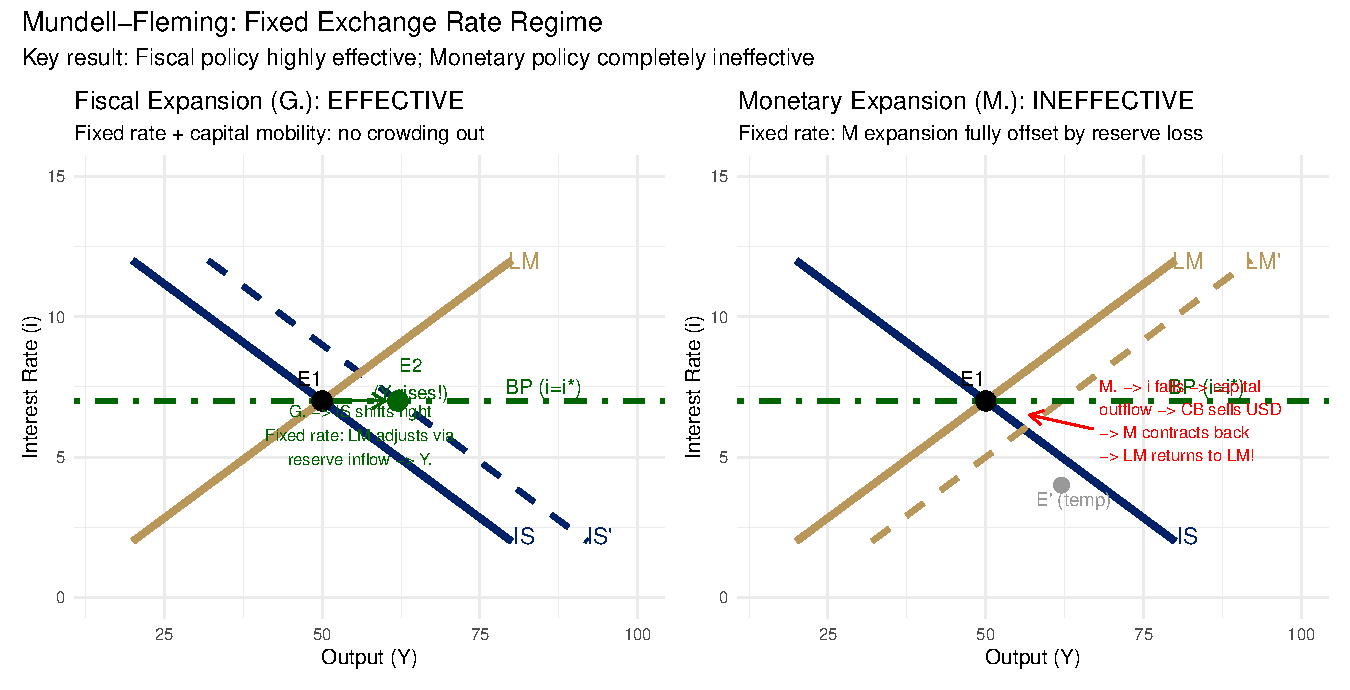
\includegraphics[keepaspectratio]{Lecture12_Forex_Market_files/figure-beamer/fig-mf-fixed-1.pdf}}

}

\caption{\label{fig-mf-fixed}Mundell-Fleming Fixed Rate: Fiscal
Expansion is Effective; Monetary Expansion is Not Source: Author's
illustration after Mundell (1963) and Fleming (1962).}

\end{figure}%

\textbf{Mathematical mechanism --- why monetary policy fails under fixed
rate:}

Under fixed \(e\): \(M\uparrow \Rightarrow i\downarrow \Rightarrow\)
capital outflow \(\Rightarrow\) BoP deficit \(\Rightarrow\) CB sells
reserves \(\Rightarrow M\) contracts back to original level.

\textbf{Agricultural policy implication:} Under a fixed rate, only
government spending (e.g., irrigation subsidies, MSP support operations,
fertiliser subsidies) can stimulate the farm economy --- not RBI rate
cuts. The RBI is powerless to lower borrowing costs for farmers if the
exchange rate is pegged.
\end{frame}

\begin{frame}{MF Model: Flexible Exchange Rate --- Monetary Effective,
Fiscal Crowded Out}
\phantomsection\label{mf-model-flexible-exchange-rate-monetary-effective-fiscal-crowded-out}
\begin{figure}

\centering{

\pandocbounded{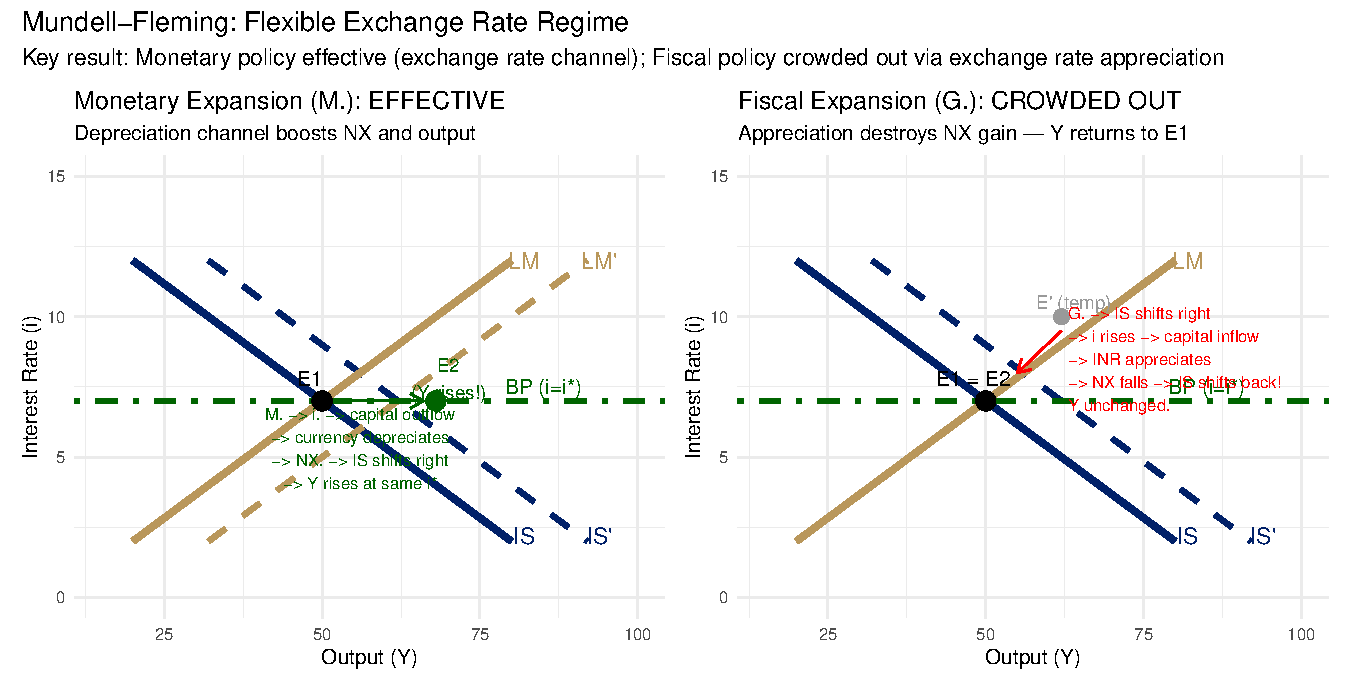
\includegraphics[keepaspectratio]{Lecture12_Forex_Market_files/figure-beamer/fig-mf-flexible-1.pdf}}

}

\caption{\label{fig-mf-flexible}Mundell-Fleming Flexible Rate: Monetary
Policy Effective; Fiscal Policy Crowded Out via Exchange Rate Source:
Author's illustration after Mundell (1963) and Fleming (1962).}

\end{figure}%

\textbf{Mathematical mechanism --- fiscal crowding out under flexible
rate:}

Under flexible \(e\):
\(G\uparrow \Rightarrow Y\uparrow \Rightarrow M_d\uparrow \Rightarrow i\uparrow \Rightarrow\)
capital inflow \(\Rightarrow\) INR appreciates
\(\Rightarrow NX\downarrow \Rightarrow Y\) falls back

\textbf{Agricultural implication under flexible rate:} RBI rate cuts
(monetary easing) boost agri exports via INR depreciation; fiscal
spending on agriculture (e.g., PM-KISAN, PMFBY) may be partially crowded
out by INR appreciation --- reducing export competitiveness even as
domestic support rises.
\end{frame}

\begin{frame}{Mundell-Fleming: Policy Effectiveness Summary}
\phantomsection\label{mundell-fleming-policy-effectiveness-summary}
\begin{longtable}[]{@{}
  >{\raggedright\arraybackslash}p{(\linewidth - 4\tabcolsep) * \real{0.2353}}
  >{\raggedright\arraybackslash}p{(\linewidth - 4\tabcolsep) * \real{0.3235}}
  >{\raggedright\arraybackslash}p{(\linewidth - 4\tabcolsep) * \real{0.4412}}@{}}
\toprule\noalign{}
\begin{minipage}[b]{\linewidth}\raggedright
Policy
\end{minipage} & \begin{minipage}[b]{\linewidth}\raggedright
Fixed Rate
\end{minipage} & \begin{minipage}[b]{\linewidth}\raggedright
Flexible Rate
\end{minipage} \\
\midrule\noalign{}
\endhead
Fiscal expansion (G↑) & \textbf{Effective} --- no crowding out, LM
adjusts via reserves & \textbf{Ineffective} --- crowded out by exchange
rate appreciation \\
Monetary expansion (M↑) & \textbf{Ineffective} --- fully offset by
reserve loss & \textbf{Effective} --- works via exchange rate
depreciation channel \\
Mechanism & Reserve flows maintain fixed e & Exchange rate adjusts to
maintain BoP \\
\bottomrule\noalign{}
\end{longtable}

\textbf{Mundell's insight (Nobel Prize 2000):} The exchange rate regime
determines which instruments of macroeconomic policy are effective.
India's managed float means both instruments have \emph{partial}
effectiveness --- neither fully effective nor fully neutralised.

\textbf{Agricultural policy implication:} Under India's managed float,
RBI rate reductions (monetary easing) can boost INR exports through
depreciation --- but the effect is partial and conditional on RBI
allowing the exchange rate to move. When RBI intervenes to prevent
depreciation (to fight inflation), the monetary transmission via
exchange rate is blocked.
\end{frame}

\begin{frame}{India's Forex Reserves: From Crisis to Abundance}
\phantomsection\label{indias-forex-reserves-from-crisis-to-abundance}
\begin{figure}

\centering{

\pandocbounded{
\includegraphics[keepaspectratio]{Lecture12_Forex_Market_files/figure-beamer/fig-forex-reserves-1.pdf}}

}

\caption{\label{fig-forex-reserves}India's Forex Reserves (USD billion)
and Import Cover (months), 2000--2024 Source: RBI, Database on Indian
Economy (DBIE).}

\end{figure}%

\[\text{RBI's forex reserves} \approx \$645\text{B (FY2024)} \approx 11\text{ months of import cover}\]

\textbf{Safety threshold} = 3 months (Guidotti-Greenspan rule). India's
current buffer gives the RBI substantial firepower to defend the rupee
in times of global turbulence. The \$645B reserve stockpile is the
direct product of 30 years of managed-float reserve accumulation --- a
deliberate policy choice to never repeat 1991.
\end{frame}

\begin{frame}{RBI and India's Managed Float}
\phantomsection\label{rbi-and-indias-managed-float}
\textbf{How RBI intervenes:}

\begin{itemize}
\tightlist
\item
  \textbf{Depreciation prevention} (INR falls too fast): RBI
  \textbf{sells USD} from reserves, absorbing rupees → reduces money
  supply → supports INR
\item
  \textbf{Appreciation prevention} (INR rises too fast): RBI
  \textbf{buys USD}, injecting rupees → increases money supply → weakens
  INR
\end{itemize}

\textbf{Sterilization mechanism:}

\[\Delta \text{Reserves} + \Delta \text{Domestic Credit} = \Delta M\]

When RBI buys USD → \(\Delta M\) (base money rises) → RBI sells G-secs
(government securities) to sterilize --- absorbing ₹ and keeping money
supply neutral.

\textbf{Two-way intervention (managed float):}

\begin{itemize}
\tightlist
\item
  \textbf{Sell USD} when INR weakens sharply (e.g., 2022)
\item
  \textbf{Buy USD} when INR strengthens too fast (e.g., 2021)
\item
  Sterilisation uses liquidity operations (OMOs, reverse repo, etc.)
\end{itemize}

\textbf{RBI's two-way intervention evidence:} - FY2021: Net purchases
\textasciitilde\$67B (preventing appreciation during COVID capital
inflows) - FY2022--23: Net sales \textasciitilde\$100B (preventing
excessive depreciation) - IMF and US Treasury classification: India is
\textbf{NOT} a currency manipulator --- two-way intervention
distinguishes managed float from competitive devaluation.
\end{frame}

\begin{frame}{The Forward Exchange Market (idea)}
\phantomsection\label{the-forward-exchange-market-idea}
\begin{itemize}
\tightlist
\item
  A \textbf{forward} locks in an exchange rate today for a future date
\end{itemize}

\[\text{Forward premium} = \frac{F - E}{E} \times \frac{12}{n} \times 100\%\]

Example (3-month): \(E=₹83.5/\$\), \(F=₹84.2/\$\) → premium ≈
\textbf{3.35\% p.a.}
\end{frame}

\begin{frame}{Who uses forwards (agri context)}
\phantomsection\label{who-uses-forwards-agri-context}
\begin{itemize}
\tightlist
\item
  Large exporters: lock in INR realisation on USD receipts
\item
  Large importers (edible oils, fertiliser): lock in INR cost of USD
  payments
\item
  Small farmers/FPOs have limited direct access (scale + documentation)
\end{itemize}
\end{frame}

\begin{frame}{Hedging with a forward (diagram)}
\phantomsection\label{hedging-with-a-forward-diagram}
\begin{figure}

\centering{

\pandocbounded{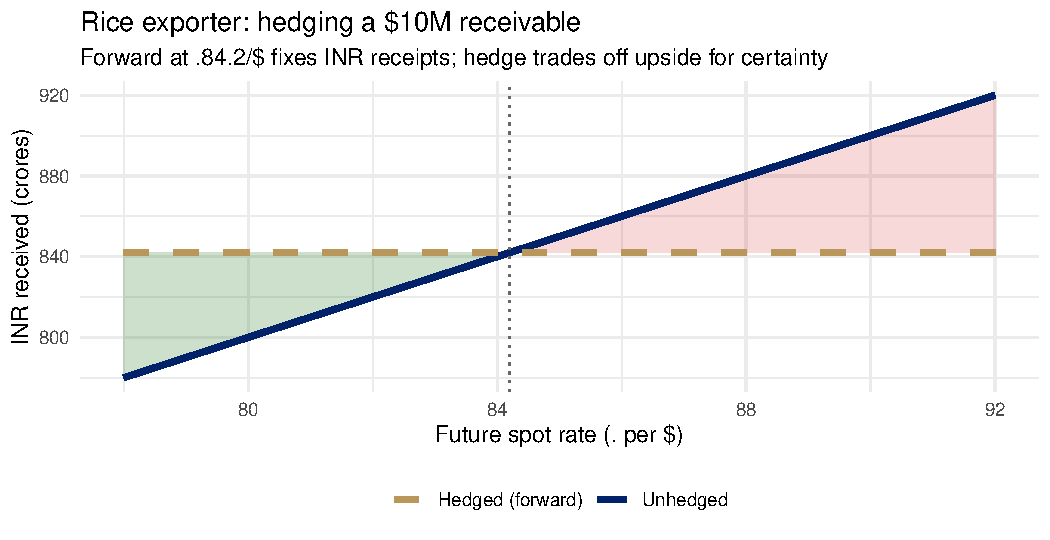
\includegraphics[keepaspectratio]{Lecture12_Forex_Market_files/figure-beamer/fig-hedging-1.pdf}}

}

\caption{\label{fig-hedging}Hedging with a forward: exporter locks in
INR receipts at a forward rate. Source: Author's illustration.}

\end{figure}%
\end{frame}

\begin{frame}{Access gap: OTC vs futures}
\phantomsection\label{access-gap-otc-vs-futures}
\begin{itemize}
\tightlist
\item
  OTC forwards typically require large minimum sizes
\item
  Exchange-traded currency futures have smaller lot sizes but require
  margin + daily mark-to-market
\end{itemize}

In practice, hedging is much easier for large firms than for small
farmers and FPOs.
\end{frame}

\begin{frame}{Exchange Rate Pass-Through}
\phantomsection\label{exchange-rate-pass-through}
\textbf{Definition:} The \textbf{pass-through coefficient} \(\psi\)
measures how much of an exchange rate change is reflected in domestic
import prices.

\[\psi = \frac{\% \Delta P^{import}}{\% \Delta e}\]

\begin{itemize}
\tightlist
\item
  If \(\psi = 1\) (\textbf{complete pass-through}): 10\% INR
  depreciation → 10\% rise in import prices (exporters maintain
  foreign-currency price)
\item
  If \(\psi < 1\) (\textbf{incomplete}): foreign exporters absorb some
  of the change in their margins (especially for branded/differentiated
  goods)
\end{itemize}

\textbf{General formula:}

\[\Delta P^{import} = \psi \cdot \Delta e + \text{world price change}\]

\textbf{India estimates:}

\begin{itemize}
\tightlist
\item
  \textbf{Edible oil:} \(\psi \approx 0.7\)--\(0.85\) (high --- palm oil
  is homogeneous, world price sets import price)
\item
  \textbf{Manufactured imports:} \(\psi \approx 0.4\)--\(0.6\) (lower
  --- brand and quality differentiation)
\item
  \textbf{Petroleum products:} \(\psi \approx 0.9\) (nearly complete ---
  global commodity)
\end{itemize}

\textbf{India's edible oil channel:}

₹10 depreciation per dollar (e.g., ₹75 → ₹85) → palm oil domestic price
rises \textasciitilde₹8--9 per litre (pass-through ≈ 80\%). At India's
\textbf{20 million tonne} annual edible oil consumption
(\textasciitilde1.4 billion litres), a ₹9/litre rise = ₹12,600 crore
additional annual cost for consumers. This is a direct \textbf{food
security and inflation} consequence of INR depreciation --- exchange
rate policy and food price policy are inseparable.
\end{frame}

\begin{frame}{INR Depreciation and Agricultural Exports}
\phantomsection\label{inr-depreciation-and-agricultural-exports}
\begin{figure}

\centering{

\pandocbounded{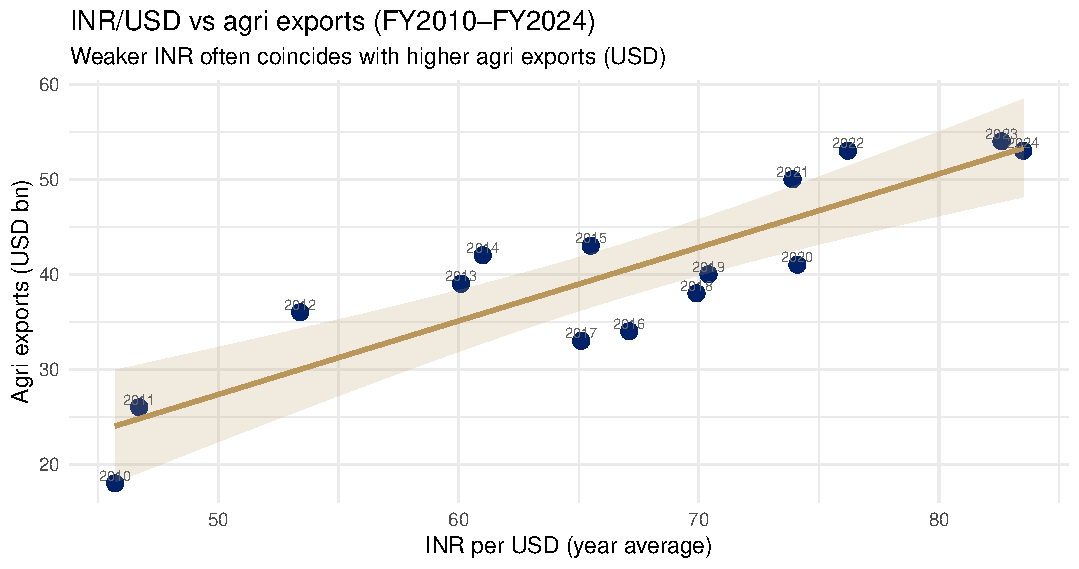
\includegraphics[keepaspectratio]{Lecture12_Forex_Market_files/figure-beamer/fig-inr-agri-exports-1.pdf}}

}

\caption{\label{fig-inr-agri-exports}INR/USD Rate vs India's
Agricultural Export Value (FY2010--FY2024) Source: RBI (exchange rate);
APEDA / DGCI\&S (export value).}

\end{figure}%

\textbf{Interpretation:} Correlation \(r \approx +0.85\) --- weaker INR
generally associated with higher agri exports in USD terms (and much
higher in INR terms).

\textbf{Caveat:} Causation runs both ways, and global demand also
matters (e.g., China's soybean demand, Middle East rice demand). The
correlation reflects both the price competitiveness effect and the
common driver of global commodity cycles.

\textbf{2013--14 rice export boom:} INR fell from ₹53 → ₹61
(depreciation of 15\%). India's rice exports rose 35\% in USD terms ---
India became the world's largest rice exporter, displacing Thailand.

\textbf{Competitiveness arithmetic:}

At ₹83/\$ vs ₹75/\$: Indian rice is effectively \textbf{10.7\% cheaper}
for foreign buyers (since they pay in USD, and more INR are now received
per dollar exported). This is a direct price competitiveness gain ---
equivalent to a 10.7\% export subsidy, but achieved through exchange
rate movement rather than fiscal expenditure.
\end{frame}

\begin{frame}{India's edible oil vulnerability (headline)}
\phantomsection\label{indias-edible-oil-vulnerability-headline}
\begin{itemize}
\tightlist
\item
  Imports ≈ \textbf{14--16 Mt} per year (large import dependence)
\item
  Major sources: Indonesia/Malaysia (palm), Argentina/Brazil (soy),
  Black Sea (sunflower)
\item
  Exchange rate movements feed into domestic cooking-oil inflation
\end{itemize}
\end{frame}

\begin{frame}{Exchange rate arithmetic (simple)}
\phantomsection\label{exchange-rate-arithmetic-simple}
\begin{itemize}
\tightlist
\item
  If world palm oil price is fixed in USD, a weaker INR raises the
  ₹/tonne cost
\item
  Example: moving from \textbf{₹75/\$ → ₹85/\$} raises rupee cost by
  \textasciitilde{}\textbf{13\%} (holding USD price constant)
\end{itemize}
\end{frame}

\begin{frame}{Policy levers and the ``duty floor'' problem}
\phantomsection\label{policy-levers-and-the-duty-floor-problem}
\begin{itemize}
\tightlist
\item
  Duty cuts can cushion price spikes, but \textbf{0\% is the floor}
\item
  Once duties are cut, INR depreciation still passes through to prices
\item
  Edible oils therefore link exchange rates to \textbf{food inflation}
\end{itemize}

Edible oils are the cleanest channel where exchange rate policy becomes
food policy.
\end{frame}

\begin{frame}{Managing Currency Risk in Agricultural Trade}
\phantomsection\label{managing-currency-risk-in-agricultural-trade}
\textbf{Agri Exporters} \emph{(risk: INR appreciates, reducing INR
revenue)}

\begin{itemize}
\tightlist
\item
  \textbf{Forward sales:} lock in ₹/\$ today for future USD receipt ---
  eliminate downside but sacrifice upside
\item
  \textbf{Export credit in USD (ECB):} borrow in USD, repay with export
  proceeds --- no currency conversion needed
\item
  \textbf{Put options on USD:} right to sell USD at floor price ---
  limits downside while retaining upside
\end{itemize}

\textbf{Agri Importers} \emph{(risk: INR depreciates, raising ₹ cost)}

\begin{itemize}
\tightlist
\item
  \textbf{Forward purchases:} lock in ₹/\$ for future USD payment ---
  certainty on import cost
\item
  \textbf{Call options on USD:} right to buy USD at ceiling price ---
  caps cost if INR weakens
\end{itemize}

\note{\textbf{Other exporter tools:} - \textbf{Natural hedge:} match USD
receivables with USD payables --- if exporter also imports inputs in USD
- \textbf{Invoice in INR} (for niche/branded exports --- Darjeeling tea,
GI products --- where buyer accepts INR pricing)

\textbf{Other importer tools:} - \textbf{Stock more when rate is
favorable:} build inventory at ₹75/\$ to avoid exposure at ₹83/\$ -
\textbf{Rupee-denominated import contracts:} India negotiating with some
suppliers (UAE, Russia) for INR-denominated trade

\textbf{Policy gap --- the small farmer problem:} Most small farmers and
village-level exporters have NO access to these instruments. The entire
forex risk is absorbed upstream by the aggregator/exporter, who
discounts the farmgate price as compensation.}
\end{frame}

\begin{frame}{BoP and the Current Account Deficit: The Agricultural
Connection}
\phantomsection\label{bop-and-the-current-account-deficit-the-agricultural-connection}
\textbf{BoP structure:}

\[\text{Current Account} + \text{Capital Account} + \text{Financial Account} = 0\]

India's current account deficit (CAD) averages \textbf{1.5--2.5\% of
GDP} (relatively moderate by emerging market standards).

\textbf{Main CAD drivers:}

\[CAD = TB_{merch} + TB_{services} + \text{Remittances} + \text{Primary income}\]

FY2024 approximate:
\(-\$300B + \$150B + \$100B + (-\$30B) \approx -\$80B \text{ CAD}\)

\textbf{Agricultural trade balance --- a current account bright spot:}

\begin{itemize}
\tightlist
\item
  India's agri trade balance: typically a \textbf{surplus of
  \textasciitilde\$20--25B} (FY2024: \textasciitilde\$25B net)
\item
  This surplus partially offsets the oil import bill
  (\textasciitilde\$200B) and gold imports (\textasciitilde\$40B)
\end{itemize}

\textbf{Agriculture's role in India's BoP:}

India's agricultural export surplus (\textasciitilde\$25B in FY2024) is
a meaningful contributor to current account balance. The major items:
rice (\textasciitilde\$10B), spices (\textasciitilde\$4B), sugar
(\textasciitilde\$3B), marine products (\textasciitilde\$7B), cotton
(\textasciitilde\$2B). Exchange rate depreciation that boosts agri
exports \textbf{directly helps the BoP} by expanding this surplus ---
which in turn reduces pressure on the RBI to defend the rupee.

\textbf{The policy feedback loop:} Weaker INR → higher agri exports →
better BoP → less reserve depletion → less pressure on INR → partial
self-correction. This is the open economy automatic stabiliser at work.
\end{frame}

\begin{frame}{Key Takeaways: Lecture 12}
\phantomsection\label{key-takeaways-lecture-12}
\textbf{Five core concepts from Lecture 12:}

\begin{enumerate}
\item
  \textbf{Exchange rate regimes:} Free float (USA), managed float
  (India), fixed (Gulf). India's managed float (post-1993) preserves
  partial monetary independence at the cost of active reserve management
  (\$645B stockpile).
\item
  \textbf{Impossible Trinity:} Cannot have all three of fixed rate +
  free capital + monetary independence. India chooses partial versions
  of all three --- a pragmatic compromise that gives flexibility without
  full commitment to any extreme.
\item
  \textbf{Mundell-Fleming model:}

  \begin{itemize}
  \tightlist
  \item
    \emph{Fixed rate}: Fiscal policy effective
    (\(G\uparrow \Rightarrow Y\uparrow\)); Monetary policy ineffective
    (\(M\uparrow\) offset by reserve loss)
  \item
    \emph{Flexible rate}: Monetary policy effective
    (\(M\uparrow \Rightarrow e\uparrow \Rightarrow NX\uparrow \Rightarrow Y\uparrow\));
    Fiscal crowded out by appreciation
  \end{itemize}
\item
  \textbf{Hedging:} Forward contracts lock in exchange rate for future
  transactions; essential for large agri exporters/importers. CIP
  ensures forward premium = interest differential. Small farmers cannot
  access these instruments --- a key equity gap.
\item
  \textbf{Agriculture--exchange rate nexus:} Depreciation helps
  rice/cotton/spice exporters (direct competitiveness); hurts edible
  oil/fertiliser importers (cost inflation); RBI's managed float
  attempts to balance these competing interests through two-way
  intervention.
\end{enumerate}
\end{frame}

\begin{frame}{Exchange Rates as Agricultural Trade Policy}
\phantomsection\label{exchange-rates-as-agricultural-trade-policy}
\textbf{Exchange rate policy IS trade policy in disguise:}

A country that keeps its currency undervalued effectively
\textbf{subsidises all its exports} and \textbf{taxes all its imports}
--- without any WTO-notifiable expenditure.

\textbf{China's managed undervaluation (2000s):}

\begin{itemize}
\tightlist
\item
  RMB/USD held artificially low through massive reserve accumulation
  (\$3T+)
\item
  Made Chinese agri exports (garlic, processed food, aquaculture) highly
  competitive globally
\item
  Undercut Indian agri exporters in third markets --- without any
  explicit subsidy
\end{itemize}

\textbf{Brazil's floating BRL --- competitive depreciation by market:}

\begin{itemize}
\tightlist
\item
  BRL/USD fell \textasciitilde50\% in 2015--16 (from BRL 2.5 → BRL
  4.0/\$)
\item
  Made Brazilian soy, beef, chicken dramatically cheaper in USD terms
\item
  Directly hurt Indian soy farmers and agri exporters in overlapping
  markets
\item
  India had no ``WTO case'' --- Brazil's depreciation was market-driven,
  not policy-directed
\end{itemize}

\textbf{India's REER concern:}

\begin{itemize}
\tightlist
\item
  If India's \textbf{Real Effective Exchange Rate (REER)} rises (INR
  appreciates in real terms relative to trading partners), agri exports
  face headwind regardless of domestic MSP levels
\item
  REER = nominal exchange rate × (domestic price level / foreign price
  level) --- captures competitiveness
\item
  India's REER has trended upward since 2014 (relatively higher
  inflation than trading partners + nominal rupee stability)
\end{itemize}

\textbf{WTO and exchange rates --- a critical gap:}

WTO disciplines \textbf{agricultural subsidies} (AoA Agreement) but does
\textbf{NOT} discipline exchange rate policy. Countries can gain large
competitive advantages in agricultural trade through currency policy ---
without violating WTO commitments. This is a major structural asymmetry
in international trade rules: a \$1B MSP subsidy is notifiable and
challengeable; a \$50B reserve accumulation that undervalues the
currency is not. The IMF (not WTO) has jurisdiction on exchange rate
manipulation --- but enforcement is weak.
\end{frame}

\begin{frame}{Next Lecture: Balance of Payments Analysis}
\phantomsection\label{next-lecture-balance-of-payments-analysis}
\textbf{Lecture 13 (July 18, 2026):} \emph{Balance of Payments:
Structure, Adjustment, and Agricultural Trade}

We will cover:

\begin{itemize}
\tightlist
\item
  Current account, capital account, financial account structure
\item
  BoP adjustment mechanisms: automatic vs policy-driven
\item
  \textbf{Marshall-Lerner condition:} when does depreciation improve the
  trade balance?
\item
  \textbf{J-curve effect:} short-run vs long-run response to
  depreciation
\item
  India's current account deficit: causes and sustainability
\end{itemize}

\note{\begin{itemize}
\tightlist
\item
  Agricultural trade's role in India's BoP (FY2024: \textasciitilde\$25B
  surplus)
\end{itemize}

\textbf{Bridge from today:} Today we studied what exchange rate regime
India operates under, how policy works under different regimes
(Mundell-Fleming), how RBI manages the float, and hedging implications.

\emph{Reading: Salvatore Ch 12--13; Appleyard Ch 18--19}}
\end{frame}

\section{Appendix}\label{appendix}

\begin{frame}{Additional Resources}
\phantomsection\label{additional-resources}
\textbf{Further reading}

\begin{itemize}
\tightlist
\item
  Salvatore, \emph{International Economics} (relevant chapters)
\item
  Appleyard \& Field, \emph{International Economics} (relevant chapters)
\end{itemize}

\textbf{Key data sources}

\begin{itemize}
\tightlist
\item
  DGCI\&S: merchandise trade
\item
  RBI: exchange rates + BoP
\item
  APEDA: agricultural export statistics
\item
  WTO: tariff + trade databases
\end{itemize}
\end{frame}




\end{document}
